\subsection{Crossing BT}
\label{sec:Crossing-BT-impl}
    This tree is used for the main decision-making process. It is the third sub-tree to be executed, and the only one to be executed repeatedly.\\
    In multiple nodes we will use information about the detected vehicles, and collision parameters for each vehicle. Therefore, we first need to define the data structures used to store this information.\\\\
    \bfc{Vehicle data}\\
        The data structure for storing the information about the detected vehicles is defined as follows:
        \begin{lstlisting}[language=C++, caption={Vehicle data structure}, label={lst:vehicle_data}]
            struct vehicle_info {
                int id;
                double x_pos;
                double y_pos;
                double x_dot;
                double y_dot;
                double x_ddot;
                double y_ddot;
                double length;
                double width;
            };
            struct vehicles_data {
                int num_vehicles;
                std::vector<vehicle_info> data;
            };
        \end{lstlisting}
        The first struct \texttt{vehicle\_info} is used to store the information about single detected vehicle. The position of the vehicle is expressed in relation to the robot's frame. The robot frame means, the center of the robot is the origin of the coordinate system. The $x$-axis points forward from robot and the $y$-axis points to the left.\\
        The second struct \texttt{vehicles\_data} is used to store the \texttt{vehicle\_info} structs of all detected vehicles.\\\\
    \bfc{Collision data}\\
        The data structure for storing the collision parameters has the following definition:
        \begin{lstlisting}[language=C++, caption={Collision data structure}, label={lst:collision_data}]
            struct collision_info {
                int car_id;
                double v_front;
                double v_back;
                bool collide;
                bool collide_stop;
            };
            struct collisions_data {
                int num_collisions;
                std::vector<collision_info> data;
            };
        \end{lstlisting}
        The first struct \texttt{collision\_data} is used to store the collision parameters for single vehicle.\\
        The \texttt{v\_front} and \texttt{v\_back} variables are the velocities of the robot to come into contact with the front or back of the vehicle. The figure \ref{fig:collision} shows the contact points we are calculating the velocities for. The figure is explained in the next part.\\
        The \texttt{collide} variable is a boolean value that tells us if the robot is going to collide with the vehicle. It is calculated based on the current velocities of the robot and the vehicle.\\
        The second struct \texttt{collisions\_data} is used to store the information about collisions with all detected vehicles.\\\\
    \bfc{Used units}\\
        We use these units for the measured and calculated parameters:
        \begin{itemize}
            \item \textbf{Position} -- meters $[\si{\m}]$
            \item \textbf{Time} -- seconds $[\si{\s}]$
            \item \textbf{Velocity} -- meters per second $[\si{\m\per\s}]$
            \item \textbf{Acceleration} -- meters per second squared $[\si{\m\per\square\s}]$
            \item \textbf{Dimensions} -- meters $[\si{\m}]$
        \end{itemize}
    \bfc{Calculating the collision parameters}\\
        First, we need to state the assumptions we are making in order to simplify the calculation.\\
        The first assumption is about the coordinate system we are using. We are using the robot's frame, where the robot's center is the system's origin, and all the positions are expressed in relation to this origin. The $x$-axis points forward, and the $y$-axis points to the left. We can assume this because the calculations are done periodically, and the results are only relevant for the current time step. It also simplifies the process, as the vehicle positions are already expressed in the robot frame.\\
        The second assumption is about the movement of the robot. We assume the robot is moving in a straight line with constant velocity. This is reasonable as we want the robot to be as predictable as possible, so we do not want to move the robot to the side. The assumption about the constant velocity, meaning the acceleration is zero, is also reasonable. The speeds the robot can achieve are much lower than the robot's acceleration, we can therefore neglect the acceleration.\\
        The third assumption is about the movement of the vehicle. We assume the vehicle's acceleration is constant. This is a reasonable simplification as the calculation is done periodically.\\
        The fourth assumption is that we will calculate the collision only in two dimensions. This is reasonable as the $z$-axis will not impact the occurance of a collision. Moreover, the area over which the collision can occur is relatively small, and therefore, any terrain deviation will not impact the collision significantly.\\\\
        Figure \ref{fig:collision} depicts a schematic view of the collision. There are two contact points, both on the robot and the vehicle. The first one (blue) is the point where the robot is going to collide with the front of the vehicle. The second one (red) is the point where the robot is going to collide with the back of the vehicle.\\
        \begin{figure}[ht]
            \centering
            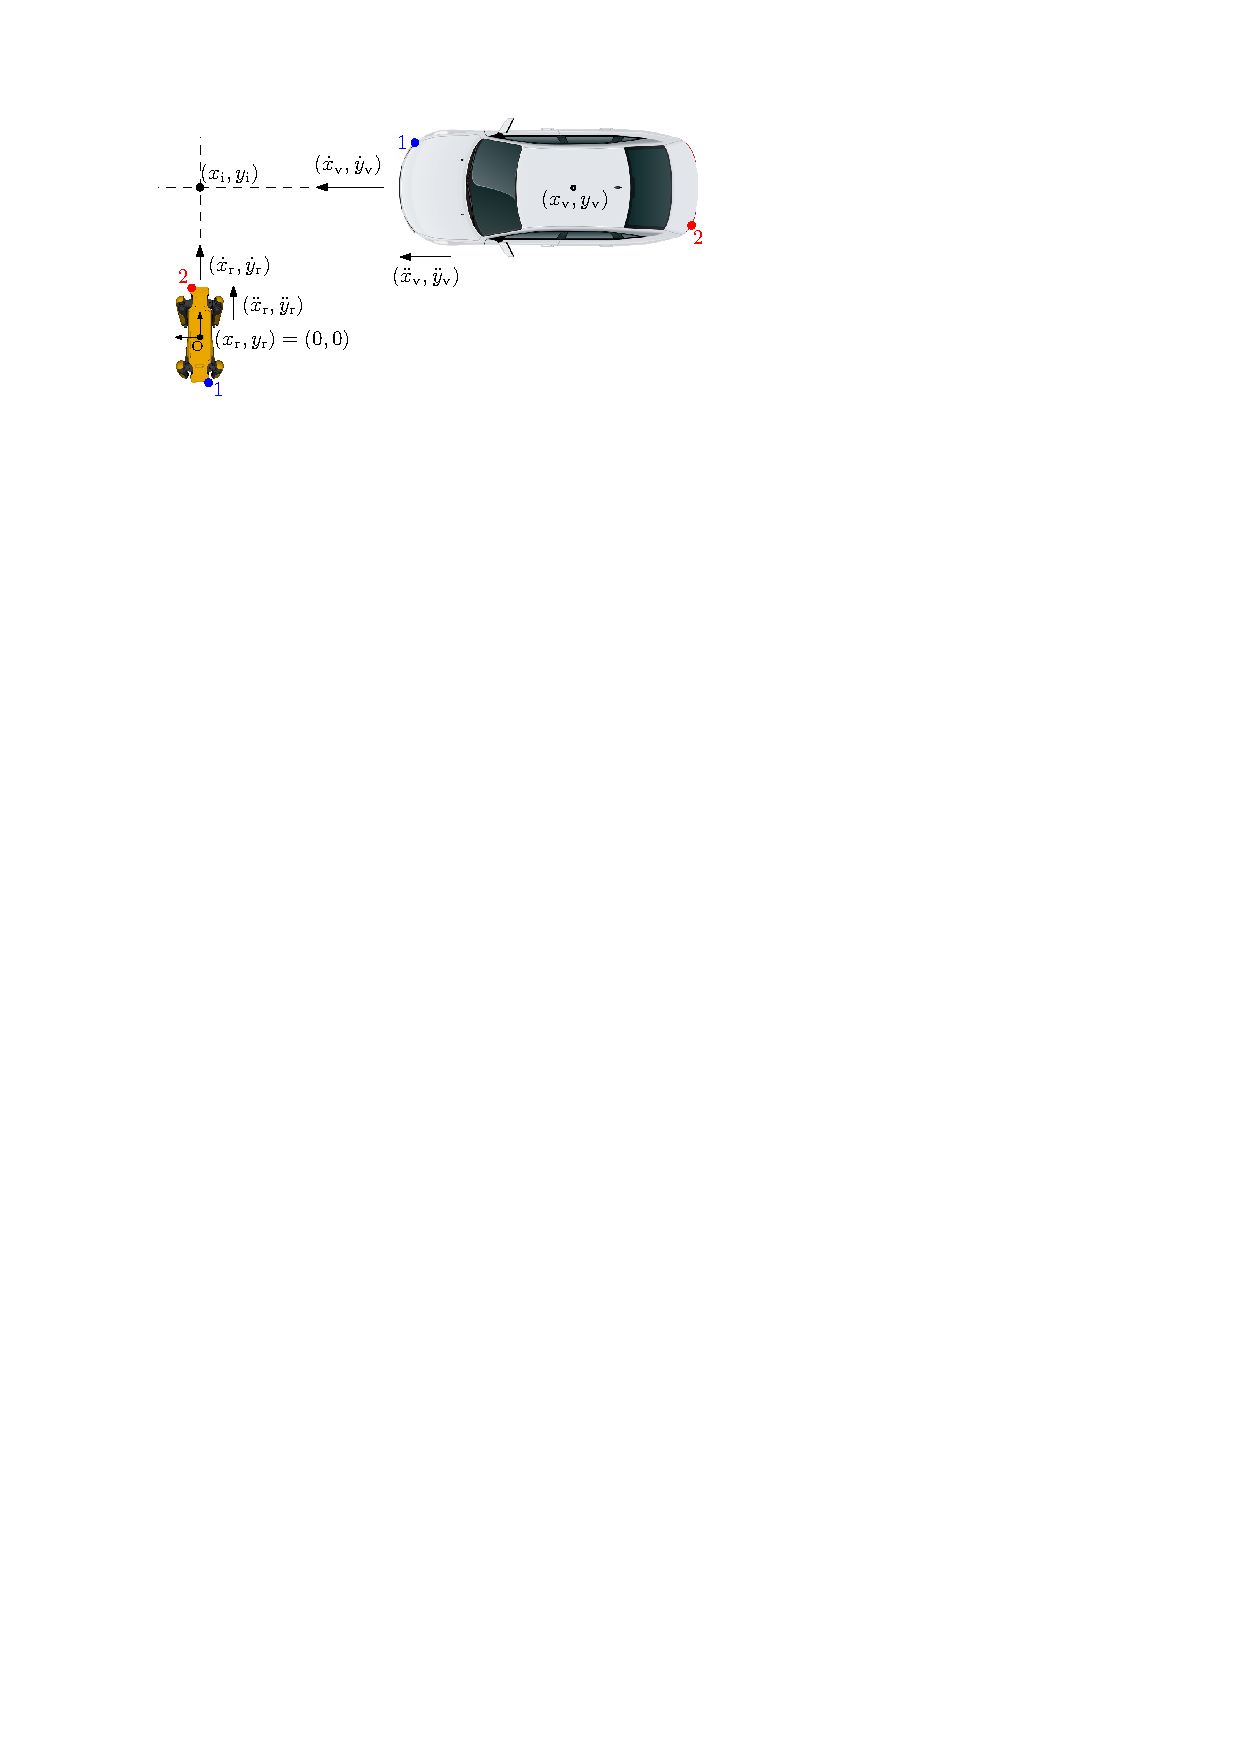
\includegraphics[height=6cm]{images/collision.pdf}
            \caption{Visualization of collision points, coordinate system, and vehicle parameters.}
            \label{fig:collision}
        \end{figure}
        \noindent For the first point, we calculate the velocity \texttt{v\_front}. This velocity depicts the minimal speed of the robot to cross in front of the vehicle. We calculate the velocity \texttt{v\_back} for the second point. This velocity depicts the maximal speed of the robot to cross behind the vehicle.\\
        The subscript \texttt{r} is used for parameters of the robot, and the subscript \texttt{v} is used for parameters of the vehicle.\\
        The calculation is divided into three parts. In the first part, we determine the starting positions of the robot and the vehicle. In the second part, we calculate the time when the vehicle will reach the intersection point $(x_{\rm{i}}, y_{\rm{i}})$. In the last part, we calculate the velocities for the robot to collide with the vehicle.\\\\
        The first part is necessary as the coordinates of both the robot and the vehicle are at the center of their respective bodies. We need to move the starting points concerning the robot's and vehicle's length and width. The starting points for the robot are calculated using these equations:
        \begin{align}
            x_{\rm{r,f}} &= \frac{l_{\rm{r}}+w_{\rm{v}}}{2},\\
            x_{\rm{r,b}} &= -\frac{l_{\rm{r}}+w_{\rm{v}}}{2},\\
            y_{\rm{r,f}} &= y_{\rm{r,b}} = 0,
        \end{align}
        where $l_{\rm{r}}$ is the length of the robot and $w_{\rm{v}}$ is the width of the vehicle.\\
        The starting points for the vehicle are calculated as follows:
        \begin{align}
            x_{\rm{v,f}} &= x_{\rm{v}} + \frac{l_{\rm{v}}+w_{\rm{r}}}{2}\cos{(\varphi_{\rm{v}})},\\
            x_{\rm{v,b}} &= x_{\rm{v}} - \frac{l_{\rm{v}}+w_{\rm{r}}}{2}\cos{(\varphi_{\rm{v}})},\\
            y_{\rm{v,f}} &= y_{\rm{v}} + \frac{l_{\rm{v}}+w_{\rm{r}}}{2}\sin{(\varphi_{\rm{v}})},\\
            y_{\rm{v,b}} &= y_{\rm{v}} - \frac{l_{\rm{v}}+w_{\rm{r}}}{2}\sin{(\varphi_{\rm{v}})},
        \end{align}
        where $\varphi_{\rm{v}} = \arctan{\left(\frac{\dot{y}_{\rm{v}}}{\dot{x}_{\rm{v}}}\right)}$ is the angle of the vehicle, $l_{\rm{v}}$ is the length of the vehicle and $w_{\rm{r}}$ is the width of the robot.\\
        We put the width of the robot to the calculation of the vehicle's starting points and vice versa because we want to flatten the dimensions of the objects. This is done to simplify the calculation of the intersection point of the robot's and vehicle's trajectory.\\
        The second part of the calculation is further divided into two parts. The reason is, that there are two possible scenarios for the calculation. We will use the general equation of motion \cite{equation_motion} for both calculations.\\
        In the first scenario, the vehicle's acceleration in the $y$-axis is zero. That means we can calculate the time using the following equations:
        \begin{align}
            t_{\rm{f}} = -\frac{y_{\rm{v,f}}}{\dot{y}_{\rm{v}}},\\
            t_{\rm{b}} = -\frac{y_{\rm{v,b}}}{\dot{y}_{\rm{v}}}.
        \end{align}
        In the second scenario, the acceleration of the vehicle in the $y$-axis is non-zero. This scenario is more probable, as vehicles rarely drive at a constant speed. In this case, the time is calculated in the following way:
        \begin{align}
            t_{\rm{f},1,2} = \frac{-\dot{y}_{\rm{v}}\pm\sqrt{\dot{y}_{\rm{v}}^2-2\ddot{y}_{\rm{v}}y_{\rm{v,f}}}}{\ddot{y}_{\rm{v}}},\\
            t_{\rm{b},1,2} = \frac{-\dot{y}_{\rm{v}}\pm\sqrt{\dot{y}_{\rm{v}}^2-2\ddot{y}_{\rm{v}}y_{\rm{v,b}}}}{\ddot{y}_{\rm{v}}}
        \end{align}
        There are two possible solutions for each time. The reason is that the vehicle may be decelerating and therefore change the direction of its travel. The interpretation of the results and the selection of the correct solution is discussed in the next section.\\
        The last part of the calculation is the calculation of the velocities. First, we need to calculate the position of the vehicle in the $x$-axis at the time of the collision. We use the general equation of motion with $t_{0}=0\:\rm{s}$:
        \begin{align}
            x_{\rm{i,f}} &= x_{\rm{v,f}} + \dot{x}_{\rm{v}}t_{\rm{f}} + \frac{1}{2}\ddot{x}_{\rm{v}}t_{\rm{f}}^2,\\
            x_{\rm{i,b}} &= x_{\rm{v,b}} + \dot{x}_{\rm{v}}t_{\rm{b}} + \frac{1}{2}\ddot{x}_{\rm{v}}t_{\rm{b}}^2.
        \end{align}
        Now we can calculate the velocities of the robot.
        \begin{align}
            \dot{x}_{\rm{r,f}} &= \frac{x_{\rm{i,f}}-x_{\rm{r,b}}}{t_{\rm{f}}},\\
            \dot{x}_{\rm{r,b}} &= \frac{x_{\rm{i,b}}-x_{\rm{r,f}}}{t_{\rm{b}}}.
        \end{align}
        The calculated velocities may be positive or negative. The interpretation is explained in the following section.\\\\
    \bfc{Interpretation of the calculated collision parameters}\\
        We will divide this section into two parts. The first part is the interpretation of the calculated time. The second part is the interpretation of the calculated velocities.\\\\
        If the calculated time is positive, the intersection point of the robot's and vehicle's trajectory is in the future. This means that the robot can collide with the vehicle without either of them changing the direction of travel.\\
        If the calculated time is negative, it means that the intersection point of the robot's and vehicle's trajectory is in the past. This means that the robot can collide with the vehicle, but only if the vehicle or the robot changes the direction of travel.\\
        The time can also be zero. This means that the robot and vehicle already collided. Therefore, we do not expect such time to arise as a result of the calculation.\\
        We may have up to two solutions when calculating the times for non-zero acceleration. If we have none, the robot's and the vehicle's trajectories do not intersect.\\
        If we have one solution, the robot's and the vehicle's trajectories intersect only once. The interpretation is that the vehicle is decelerating and will stop at the intersection point and then start reversing.\\
        If we have two solutions, the robot's and the vehicle's trajectories intersect two times. Multiple intersections could have several physical interpretations. We can interpret this as the vehicle decelerating, and therefore, changing the direction of travel after passing the intersection point. We can also interpret this as the vehicle accelerating, and therefore, the second time of the intersection is likely negative.\\
        When choosing the calculated time, we will use the following criteria. If one time is positive and the second is negative, we will use the positive time. If both times are positive, we will use the shorter time. If both times are negative, we will use the larger time (the time that is closer to the present).\\\\
        The velocities can also be positive or negative. The interpretation is similar to the one of time. Positive velocity means moving forward, while negative velocity means moving backward.\\
        While it may seem irrelevant to calculate the time and velocity for backward movement, it is essential. The reason is that some other vehicle may be moving so that the robot would collide with it. In that case, the robot will have to move backward to avoid the collision, and we need to be able to set the correct backward velocity to not collide with the first vehicle.\\\\
    \bfc{GetCars -- action node}\\
        The action node \texttt{GetCars} is responsible for obtaining information about the detected vehicles. The detection node was not yet implemented when this thesis was written. Therefore, we will use the \texttt{GetCars} node to simulate the detection of vehicles.\\
        We will subscripe to the topic \texttt{/road\_crossing/injector}. To this topic we will publish from a separate node designed solely for the purpose of simulation the detection node.\\
        The information about the detected vehicles will be stored in a static variable for later use. The variable is of the format shown in listing \ref{lst:vehicle_data}.\\\\
    \bfc{CarsInTrajectory -- condition node}\\
        This node is important for optimizing the flow of ticks in our behavior tree. The node is responsible for checking if there are any detected vehicles. If there are no vehicles we do not need to go through the calculation and decision making. This speeds up the completion of this run of the BT and allows us to start the next run sooner.\\\\
    \bfc{NotStarted -- condition node}\\
        This node is responsible for checking if the movement across the road has been started. If it has not, we need to start the movement. If it has, we may continue in it.\\\\
    \bfc{StartMovement -- action node}\\
        This node is responsible for starting the movement across the road. We will set the maximal forward linear velocity to the topic our inner static variable. This variable is responsible for storing the current velocity. We chose the maximal linear velocity as $1.2\:\si{\m\per\s}$.\\\\
    \bfc{MoveFwdFull -- action node}\\
        This node is used when no vehicles are detected and therefore we want to move the robot across the road as fast as possible. We publish the maximal forward linear velocity to the topic \texttt{/cmd\_vel}.\\\\
    \bfc{CalculateCollision -- action node}\\
        In this node we will calculate the collision parameters. We will use the formulas described earlier. The results will be stored in the inner static variables.\\
        This node will run the calculation for each vehicle independently. As each vehicle has its own ID, we will use this ID to differentiate between the vehicles. This ID will also be used to delete all the results from the inner static variable when the vehicle is no longer detected.\\\\
    \bfc{MoveFwd -- action node}\\
        This node is used when there are detected vehicles and a forward movement is possible. We will publish the forward velocity to the topic \texttt{/cmd\_vel}. The forward velocity is determined from the calculated velocities from the \texttt{CalculateCollision} node. We will set the maximal forward velocity we can, while still avoiding the collision.\\\\
    \bfc{MoveBwd -- action node}\\
        This node is used when there are detected vehicles and a backward movement is necessary. We will publish the backward velocity to the topic \texttt{/cmd\_vel}. The backward velocity is determined from the calculated velocities from the \texttt{CalculateCollision} node. We will set the minimal backward velocity we can, while still avoiding the collision.\\\\
    \bfc{StopMovement -- action node}\\
        This node is used when there is no possible movement forward without the robot colliding with a vehicle and movement back is not neccessary. We will stop the robot by publishing zero velocity to the topic \texttt{/cmd\_vel}.\\\\
    \bfc{CollisionFwdMove -- condition node}\\
        This node is used to determine whether there are vehicles in front of the robot in such a position and velocity that the robot would collide with them if it moved forward.\\\\
    \bfc{CollisionBwdMove -- condition node}\\
        This node is used to determine whether there are vehicles in such a position and velocity that the robot would collide with them if it moved backward.\\\\
    \bfc{CollisionOnStop -- condition node}\\
        This node is used to determine whether there are vehicles in such a position and velocity that the robot would collide with them if it stopped.\\\\
    \bfc{CrossingFinished -- condition node}\\
        In this node we check the current position of the robot with. If the distance of the current position from the middle of the road is greater then the half of the width of the road, we consider the crossing finished.\\
        Other condition for finishing the crossing is if the robot's distance from the starting point is greater than the width of the road.\\
        It is beneficiary to have both of these conditions as the position of the robot may be imprecise.\\\\
